% This file was created by matplotlib2tikz v0.6.15.
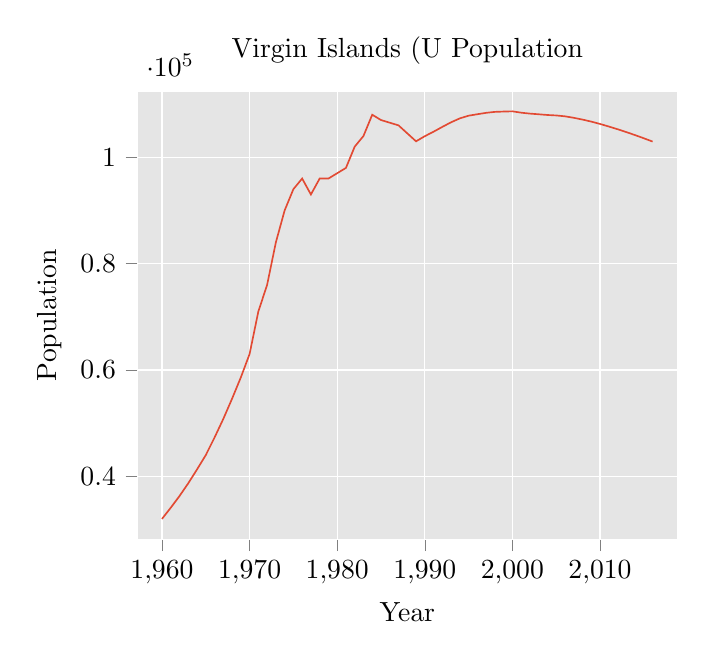
\begin{tikzpicture}

\definecolor{color0}{rgb}{0.886274509803922,0.290196078431373,0.2}

\begin{axis}[
title={Virgin Islands (U Population},
xlabel={Year},
ylabel={Population},
xmin=1957.2, xmax=2018.8,
ymin=28168.05, ymax=112470.95,
tick align=outside,
tick pos=left,
xmajorgrids,
x grid style={white},
ymajorgrids,
y grid style={white},
axis line style={white},
axis background/.style={fill=white!89.80392156862746!black}
]
\addplot [semithick, color0, forget plot]
table {%
1960 32000
1961 34100
1962 36300
1963 38700
1964 41300
1965 44000
1966 47300
1967 50800
1968 54600
1969 58600
1970 63000
1971 71000
1972 76000
1973 84000
1974 90000
1975 94000
1976 96000
1977 93000
1978 96000
1979 96000
1980 97000
1981 98000
1982 102000
1983 104000
1984 108000
1985 107000
1986 106500
1987 106000
1988 104500
1989 103000
1990 103963
1991 104807
1992 105711
1993 106577
1994 107317
1995 107817
1996 108093
1997 108355
1998 108535
1999 108596
2000 108639
2001 108386
2002 108208
2003 108085
2004 107950
2005 107863
2006 107700
2007 107423
2008 107091
2009 106707
2010 106267
2011 105784
2012 105275
2013 104737
2014 104170
2015 103574
2016 102951
};
\end{axis}

\end{tikzpicture}